%%%%%%%%%%%%%%%%%%%%%%%%%%%%%%%%%%%%%%%%%%%%%%%%%%%%%%%%%%%%%%%%%%%%%%%%
% Uni Duesseldorf
% Lehrstuhl fuer Datenbanken und Informationssysteme
% Vorlage fuer Bachelor-/Masterarbeiten
% Optimiert fuer den Original-Latex-Kompiler LATEX.EXE (LaTeX=>PS=>PDF)
%%%%%%%%%%%%%%%%%%%%%%%%%%%%%%%%%%%%%%%%%%%%%%%%%%%%%%%%%%%%%%%%%%%%%%%%
% Ueberarbeitung für pdflatex (LaTeX=>PDF)
%%%%%%%%%%%%%%%%%%%%%%%%%%%%%%%%%%%%%%%%%%%%%%%%%%%%%%%%%%%%%%%%%%%%%%%%
% Vorlage Changelog:
% 10.09.2015 (Matthias Liebeck): Nummerierung des Inhaltsverzeichnis nun römisch, Beispiel für einen Anhang eingebaut, \raggedbottom hinter sections eingefügt
%%%%%%%%%%%%%%%%%%%%%%%%%%%%%%%%%%%%%%%%%%%%%%%%%%%%%%%%%%%%%%%%%%%%%%%%
%%%% BEGINN EINSTELLUNG FUER DIE ARBEIT. UNBEDINGT ERFORDERLICH! %%%%%%%
%%%%%%%%%%%%%%%%%%%%%%%%%%%%%%%%%%%%%%%%%%%%%%%%%%%%%%%%%%%%%%%%%%%%%%%%
% Geben Sie Ihren Namen hier an:
\newcommand{\bearbeiter}{Anton Borries}

% Geben Sie hier den Titel Ihrer Arbeit an:
\newcommand{\titel}{An app for location-based feedback}

% Geben Sie das Datum des Beginns und Ende der Bachelorarbeit ein:
\newcommand{\beginndatum}{24. April 2017}
\newcommand{\abgabedatum}{26. Juli 2017}

% Geben Sie die Namen des Erst- und Zweitgutachters an:
\newcommand{\erstgutachter}{Prof.~Dr.~Michael Leuschel}
\newcommand{\zweitgutachter}{Prof.~Dr.~Stefan Conrad}

% Falls Sie die Arbeit zweiseitig ausdrucken wollen,
% benutzen Sie die folgende Zeile mit
% \AN fuer zweiseitigen Druck
% \AUS fuer einseitigen Druck
\newcommand{\zweiseitig}{\AN}

% Falls die Arbeit in englischer Sprache verfasst
% werden soll, dann benutzen Sie die folgende Zeile mit
% englisch fuer englische Sprache
% deutsch fuer deutsche Sprache
\newcommand{\sprache}{englisch}

% Hier wird eingestellt, ob es sich bei der Arbeit um eine Bachelor-
% oder Masterarbeit handelt (unpassendes auskommentieren!):
\newcommand{\arbeit}{Bachelorarbeit}
%~ \newcommand{\arbeit}{Masterarbeit}

%%%%%%%%%%%%%%%%%%%%%%%%%%%%%%%%%%%%%%%%%%%%%%%%%%%%%%%%%%%%%%%%%%%%%%%%
%%%% ENDE EINSTELLUNGEN %%%%%%%%%%%%%%%%%%%%%%%%%%%%%%%%%%%%%%%%%%%%%%%%
%%%%%%%%%%%%%%%%%%%%%%%%%%%%%%%%%%%%%%%%%%%%%%%%%%%%%%%%%%%%%%%%%%%%%%%%

% Die folgende Zeile NICHT EDITIEREN oder loeschen


%%%%%%%%%%%%%%%%%%%%%%%%%%%%%%%%%%%%%%%%%%%%%%%%%%%%%%%%%%%
% Obere Titelmakros. Editieren Sie diese Datei nur, wenn
% Sie sich ABSOLUT sicher sind, was Sie da tun!!!
% (Z.B. zum Abaendern der BA-Vorlage in eine MA-Vorlage)
% Uni Duesseldorf
% Lehrstuhl fuer Datenbanken und Informationssysteme
% Version 2.2 - 2.3.2010
%%%%%%%%%%%%%%%%%%%%%%%%%%%%%%%%%%%%%%%%%%%%%%%%%%%%%%%%%%%
\newcommand{\AN}{twoside}
\newcommand{\AUS}{}
%\newcommand{\englisch}{}
%\newcommand{\deutsch}{\usepackage[german]{babel}}

%% Die folgenden auskommentierten Optionen dienen der automatischen
%% Erkennung des Latex-Kompilers und dem Setzen der davon abhängigen
%% Einstellungen. Bei Problem z.B. mit dem Einbinden von verschiedenen
%% Grafiktypen bei Verwendung von PdfLatex oder Latex, einfach die
%% verschiedenen \usepackage(s) ausprobieren. (Mit diesen Einstellungen
%% funktionierte diese Vorlage bei der Verwenundg von latex.exe als
%% Kompiler bei den meisten Studierenden.)

%\newif\ifpdf \ifx\pdfoutput\undefineds
%\pdffalse % we are not running pdflatex
%\else
%\pdfoutput=1 % we are running pdflatex
%\pdfcompresslevel=9 % compression level for text and image;
%\pdftrue \fi

\documentclass[11pt,a4paper, \zweiseitig]{article}



%\usepackage[iso]{umlaute}
\usepackage[utf8x]{inputenc}
\usepackage{palatino} % palatino Schriftart
%\usepackage{makeidx} % um ein Index zu erstellen
\usepackage[nottoc]{tocbibind}
\usepackage[T1]{fontenc} %fuer richtige Trennung bei Umlauten
\usepackage{fancybox} % fuer die Rahmen
\usepackage{shortvrb}
\usepackage{ifthen}
\ifthenelse{\equal{\sprache}{deutsch}}{\usepackage[ngerman]{babel}}{}

\usepackage{a4wide} % ganze A4 Weite verwenden

%\ifpdf
%\usepackage[pdftex,xdvi]{graphicx}
%\usepackage{thumbpdf} %thumbs fuer Pdf
%\usepackage[pdfstartview=FitV]{hyperref} %anklickbares Inhaltsverzeichnis
%\else
%\usepackage[dvips,xdvi]{graphicx}
\usepackage{graphicx}
\usepackage{hyperref} %anklickbares Inhaltsverzeichnis
%\fi


\usepackage{color}
\usepackage{minted}



\renewcommand\fcolorbox[4][]{#4}



\usepackage{float}




%%%%%%%%%%%%%%%%%%%%%%% Massangaben fuer die Arbeit %%%%%%%%%%%%%%%
\setlength{\textwidth}{15cm}

\setlength{\oddsidemargin}{35mm}
\setlength{\evensidemargin}{25mm}

\addtolength{\oddsidemargin}{-1in}
\addtolength{\evensidemargin}{-1in}

%\makeindex

\begin{document}

%\setcounter{secnumdepth}{4} %Nummerieren bis in die 4. Ebene
%\setcounter{tocdepth}{4} %Inhaltsverzeichnis bis zur 4. Ebene

\pagestyle{headings}

\sloppy % LaTeX ist dann nicht so streng mit der Silbentrennung
%~ \MakeShortVerb{\§}

\parindent0mm
\parskip0.5em


{
\textwidth170mm
\oddsidemargin30mm
\evensidemargin30mm
\addtolength{\oddsidemargin}{-1in}
\addtolength{\evensidemargin}{-1in}

\parskip0pt plus2pt

% Die Raender muessen eventuell fuer jeden Drucker individuell eingestellt
% werden. Dazu sind die Werte fuer die Abstaende `\oben' und `\links' zu
% aendern, die von mir auf jeweils 0mm eingestellt wurden.

%\newlength{\links} \setlength{\links}{10mm}  % hier abzuaendern
%\addtolength{\oddsidemargin}{\links}
%\addtolength{\evensidemargin}{\links}

\begin{titlepage}
\vspace*{-1.5cm}
  \raisebox{17mm}{
    \begin{minipage}[t]{75mm}
      \begin{center}
        %\selectlanguage{german}
        {\Large INSTITUT FÜR INFORMATIK\\}
        {\normalsize
          Softwaretechnik und Programmiersprachen\\
        }
        \vspace{3mm}
        {\small Universitätsstr. 1 \hspace{5ex} D--40225 Düsseldorf\\}
     \end{center}
    \end{minipage}
  }
  \hfill
  
\includegraphics[width=130pt]{bilder/HHU_Logo}
  \vspace{14em}

% Titel
  \begin{center}
      	\baselineskip=55pt
    	\textbf{\huge \titel}
  	 	\baselineskip=0 pt
   \end{center}

  %\vspace{7em}

\vfill

% Autor
  \begin{center}
    \textbf{\Large
      \bearbeiter
    }
  \end{center}

  \vspace{35mm}

% Prüfungsordnungs-Angaben
  \begin{center}
    %\selectlanguage{german}

%%%%%%%%%%%%%%%%%%%%%%%%%%%%%%%%%%%%%%%%%%%%%%%%%%%%%%%%%%%%%%%%%%%%%%%%%
% Ja, richtig, hier kann die BA-Vorlage zur MA-Vorlage gemacht werden...
% (nicht mehr nötig!)
%%%%%%%%%%%%%%%%%%%%%%%%%%%%%%%%%%%%%%%%%%%%%%%%%%%%%%%%%%%%%%%%%%%%%%%%%
    {\Large \arbeit}

    \vspace{2em}

    \begin{tabular}[t]{ll}
      Beginn der Arbeit:& \beginndatum \\
      Abgabe der Arbeit:& \abgabedatum \\
      Gutachter:         & \erstgutachter \\
                         & \zweitgutachter \\
    \end{tabular}
  \end{center}

\end{titlepage}

}

%%%%%%%%%%%%%%%%%%%%%%%%%%%%%%%%%%%%%%%%%%%%%%%%%%%%%%%%%%%%%%%%%%%%%
\clearpage
\begin{titlepage}
  ~                % eine leere Seite hinter dem Deckblatt
\end{titlepage}
%%%%%%%%%%%%%%%%%%%%%%%%%%%%%%%%%%%%%%%%%%%%%%%%%%%%%%%%%%%%%%%%%%%%%
\clearpage
\begin{titlepage}
\vspace*{\fill}

\section*{Erklärung}

%%%%%%%%%%%%%%%%%%%%%%%%%%%%%%%%%%%%%%%%%%%%%%%%%%%%%%%%%%%
% Und hier ebenfalls ggf. BA durch MA ersetzen...
% (Auch nicht mehr nötig!)
%%%%%%%%%%%%%%%%%%%%%%%%%%%%%%%%%%%%%%%%%%%%%%%%%%%%%%%%%%%

Hiermit versichere ich, dass ich diese \arbeit~
selbstständig verfasst habe. Ich habe dazu keine anderen als die
angegebenen Quellen und Hilfsmittel verwendet.

\vspace{25 mm}

\begin{tabular}{lc}
Düsseldorf, den \abgabedatum \hspace*{2cm} & \underline{\hspace{6cm}}\\
& \bearbeiter
\end{tabular}

\vspace*{\fill}
\end{titlepage}

%%%%%%%%%%%%%%%%%%%%%%%%%%%%%%%%%%%%%%%%%%%%%%%%%%%%%%%%%%%%%%%%%%%%%
% Leerseite bei zweiseitigem Druck
%%%%%%%%%%%%%%%%%%%%%%%%%%%%%%%%%%%%%%%%%%%%%%%%%%%%%%%%%%%%%%%%%%%%%

\ifthenelse{\equal{\zweiseitig}{twoside}}{\clearpage\begin{titlepage}
~\end{titlepage}}{}

%%%%%%%%%%%%%%%%%%%%%%%%%%%%%%%%%%%%%%%%%%%%%%%%%%%%%%%%%%%%%%%%%%%%%
\clearpage
\begin{titlepage}

%%% Die folgende Zeile nicht ändern!
\section*{\ifthenelse{\equal{\sprache}{deutsch}}{Zusammenfassung}{Abstract}}
%%% Zusammenfassung:
Feedbacker is an app which gives users the ability to send location-based feedback. The app is available for Android and iOS. It is using Firebase as its backend.\\
This thesis presents the app and gives possible use cases. It also explains how Firebase works and in which ways it was used for Feedbacker. A special focus lies on the database function of Firebase as well as the security of the saved data as it handles sensible information in the form of the user's location.\\
Furthermore, this work also shows the process of developing an App for iOS and Android at the same time. Here, extra focus was given to the process of getting the current user's location. Also, a perspective on how to develop the App further is given.\\
As the app is not yet published, its success of it needs to be determined at a later time.



%%%%%%%%%%%%%%%%%%%%%%%%%%%%%%%%%%%%%%%%%%%%%%%%
% Untere Titelmakros. Editieren Sie diese Datei nur, wenn Sie sich
% ABSOLUT sicher sind, was Sie da tun!!!
%%%%%%%%%%%%%%%%%%%%%%%%%%%%%%%%%%%%%%%%%%%%%%%
\vspace*{\fill}
\end{titlepage}

%%%%%%%%%%%%%%%%%%%%%%%%%%%%%%%%%%%%%%%%%%%%%%%%%%%%%%%%%%%%%%%%%%%%%
% Leerseite bei zweiseitigem Druck
%%%%%%%%%%%%%%%%%%%%%%%%%%%%%%%%%%%%%%%%%%%%%%%%%%%%%%%%%%%%%%%%%%%%%
\ifthenelse{\equal{\zweiseitig}{twoside}}
  {\clearpage\begin{titlepage}~\end{titlepage}}{}
%%%%%%%%%%%%%%%%%%%%%%%%%%%%%%%%%%%%%%%%%%%%%%%%%%%%%%%%%%%%%%%%%%%%%
\clearpage \setcounter{page}{1}
\pagenumbering{roman}
\setcounter{tocdepth}{2}
\tableofcontents

%\enlargethispage{\baselineskip}
\clearpage
%%%%%%%%%%%%%%%%%%%%%%%%%%%%%%%%%%%%%%%%%%%%%%%%%%%%%%%%%%%%%%%%%%%%%
% Leere Seite, falls Inhaltsverzeichnis mit ungerader Seitenzahl und
% doppelseitiger Druck
%%%%%%%%%%%%%%%%%%%%%%%%%%%%%%%%%%%%%%%%%%%%%%%%%%%%%%%%%%%%%%%%%%%%%
\ifthenelse{ \( \equal{\zweiseitig}{twoside} \and \not \isodd{\value{page}} \)}
	{\pagebreak \thispagestyle{empty} \cleardoublepage}{\clearpage}

\pagenumbering{arabic}
\setcounter{page}{1}

%%%%%%%%%%%%%%%%%%%%%%%%%%%%%%%%%%%%%%%%%%%%%%%%%%%%%%%%%%%%%%%%%%%%%%%%
%%%% BEGINN TEXTTEIL %%%%%%%%%%%%%%%%%%%%%%%%%%%%%%%%%%%%%%%%%%%%%%%%%%%
%%%%%%%%%%%%%%%%%%%%%%%%%%%%%%%%%%%%%%%%%%%%%%%%%%%%%%%%%%%%%%%%%%%%%%%%

%%%%%%%%%%%%%%%%%%%%%%%%%%%%%%%%%%%%%%%%%%%%%%%%%%%%%%%%%%%%%%%%%%%%%%%%
% Text entweder direkt hier hinein schreiben oder, im Sinne der
% besseren Uebersichtlich- und Bearbeitbarkeit mittels \input die
% einzelnen Textteile hier einbinden.
%%%%%%%%%%%%%%%%%%%%%%%%%%%%%%%%%%%%%%%%%%%%%%%%%%%%%%%%%%%%%%%%%%%%%%%%



\section{Requirements}

\subsection{Motivation}
The original idea was to develop an App that can be used to identify certain areas in cities where users feel afraid or, in a more general term, not safe.\\
In the process of developing the app the use case was extended to not only give users the ability to mark places as unsafe but also give the option of marking a place as positive. The process lead to the app called Feedbacker.

\subsection{User groups}
The main targeted user group are individual people. Users have the option to see feedback of other users in order to see how different areas are perceived, or to get ideas what to do/where to go while planning a trip. \\
City administrations might also have interest in the gathered data to identify urban areas that could be developed further, and to determine what makes certain regions stand out in comparison to other regions.

\subsection{User Actions}
\subsubsection{Sending of Feedback}
The user has the option of sending two kinds of Feedback, positive and negative. After the user has sent the feedback it will be saved to the database containing the user's current location, the current time and the kind of feedback.

\subsubsection{Editing of Feedback}
After sending the Feedback the user has the ability to further specify it. \\
One of the main points of editing is categorizing the Feedback. The available categories are:
\begin{table}[h]
\begin{center}
\begin{tabular}{l  l}
positive & negative \\
\hline
  Places to sit & Dark Place \\
  Public/Clean Toilets & Dirty \\
  Disablity Access & Shady Group of People \\
  Public Wi-Fi & Not pedestrian friendly \\
  Place to Eat/Drink & Graffiti \\
  Nice View & \\
\end{tabular}
 \caption{Categories}\label{tab_categories}
 \label{table:categories}
\end{center}
\end{table}

To give additional information about the feedback or the place of the feedback the user can write a descriptive text. If the user decides to mark the feedback as public, other users are able to see the feedback on a map. Users can also change their feedback from positive to negative (or vice versa), for example when a place was altered or if the user clicked the wrong button when sending his feedback.

\subsection{Other Apps \& Services}
There are other apps and services which have some similarities to Feedbacker. In the following I show similarities and differences to two of those Apps.

\paragraph{Google Maps}
Google Maps has a lot of information on restaurants, shops and places in general. Users can not only rate and comment on places but Google also the option for users to add new places and enhance information like opening hours of existing places \cite{gMaps}.\\
The information is however not as prominent and readily available as it is with Feedbacker, because in Google Maps the feedback of other users is not visible at first glance.

\paragraph{wheelmap.org}
"Wheelmap is a map for finding wheelchair accessible places. The map works similar to Wikipedia: anyone can contribute and mark public places around the world according to their wheelchair accessibility. The criteria for marking places is based on a simple traffic light system". It distinguishes between 130 types of places \cite{wheel}.\\
Similar to Feedbacker, wheelmap.org shows user-submitted ratings of places directly on a map and it is also visible whether a place is rated as good or bad.\\
With Feedbacker however, users can rate places in more ways than just specialized on one feature such as wheelchair access.

\section{User Interface}
The user interface consists of a main view and a view where users can edit their Feedback.
\subsection{Main View}
The app is controlled with a main view that allows selecting from three sub-views with specific functionality. A view to send Feedback (Figure \ref{fig_send}), a map view (Figure \ref{fig_map}) and a profile view which lists the user's feedback (Figure \ref{fig_profile}). This is done via interactive buttons and controls familiar to most smartphone users.\\

\begin{figure}[H]
\minipage{0.32\textwidth}
  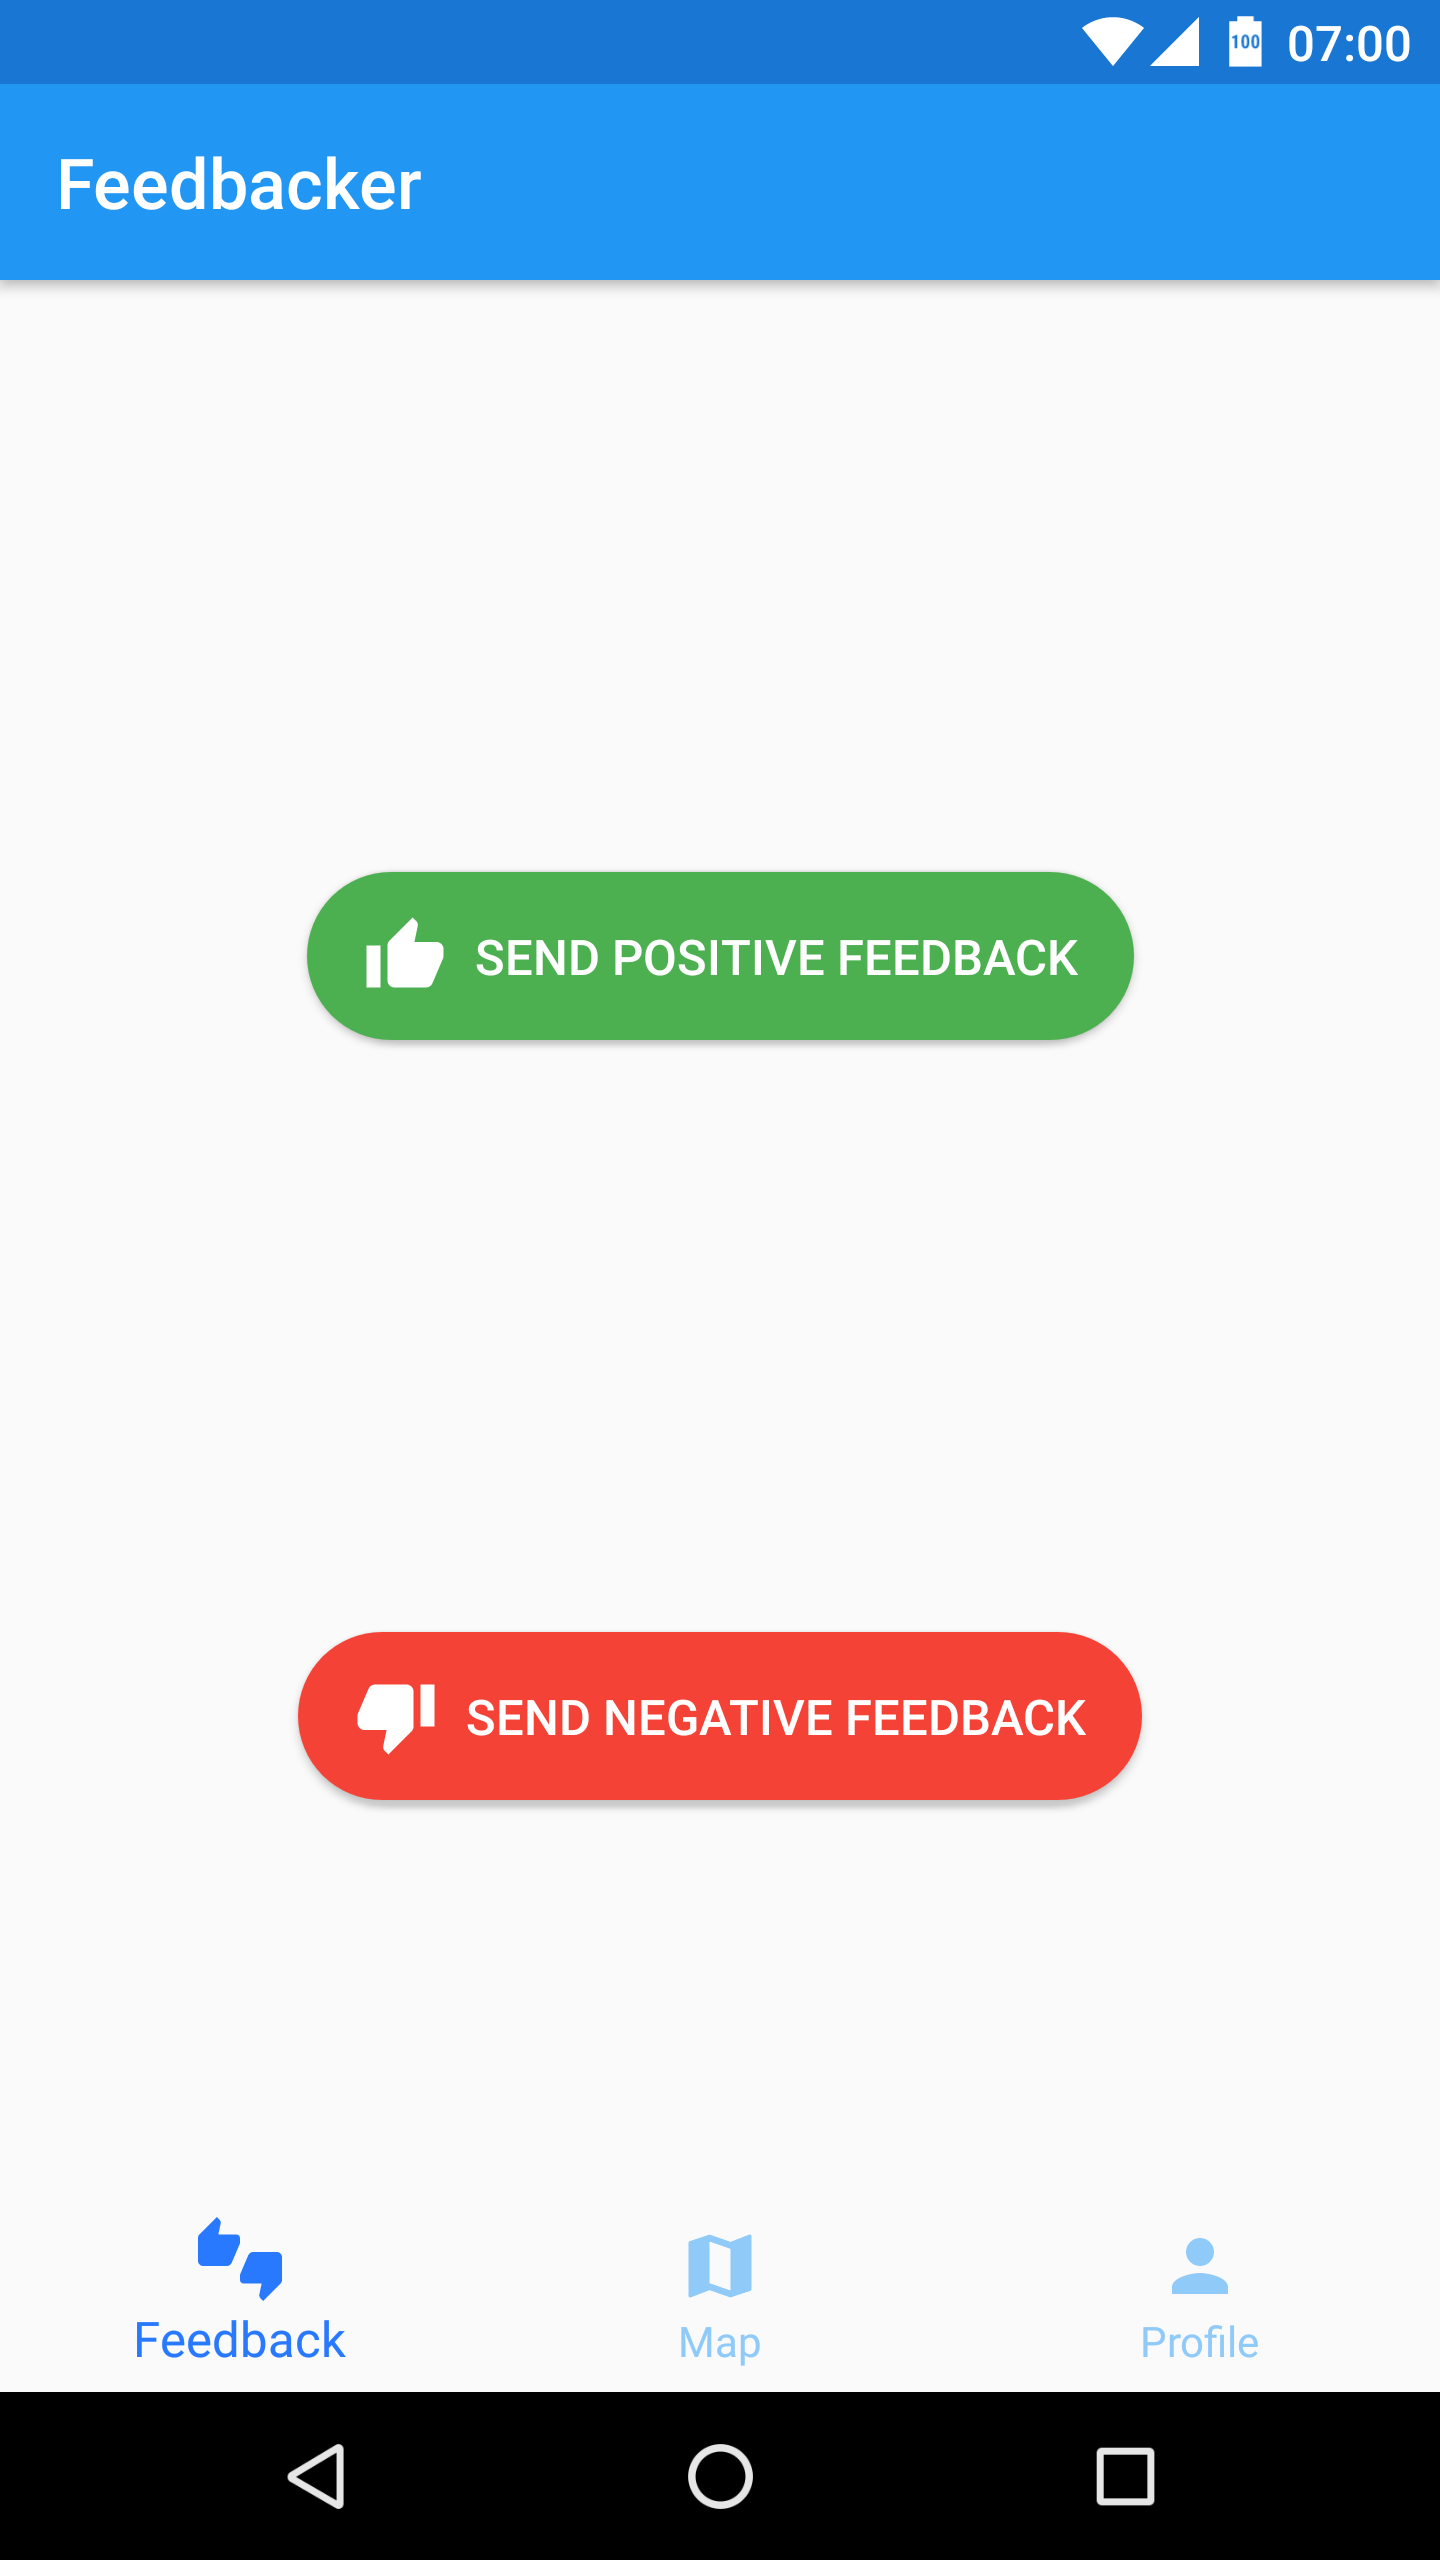
\includegraphics[width=\linewidth]{bilder/Screenshot_Send_Feedback.png}
  \caption{Feedback View Android}\label{fig_send}
\endminipage\hfill
\minipage{0.32\textwidth}
  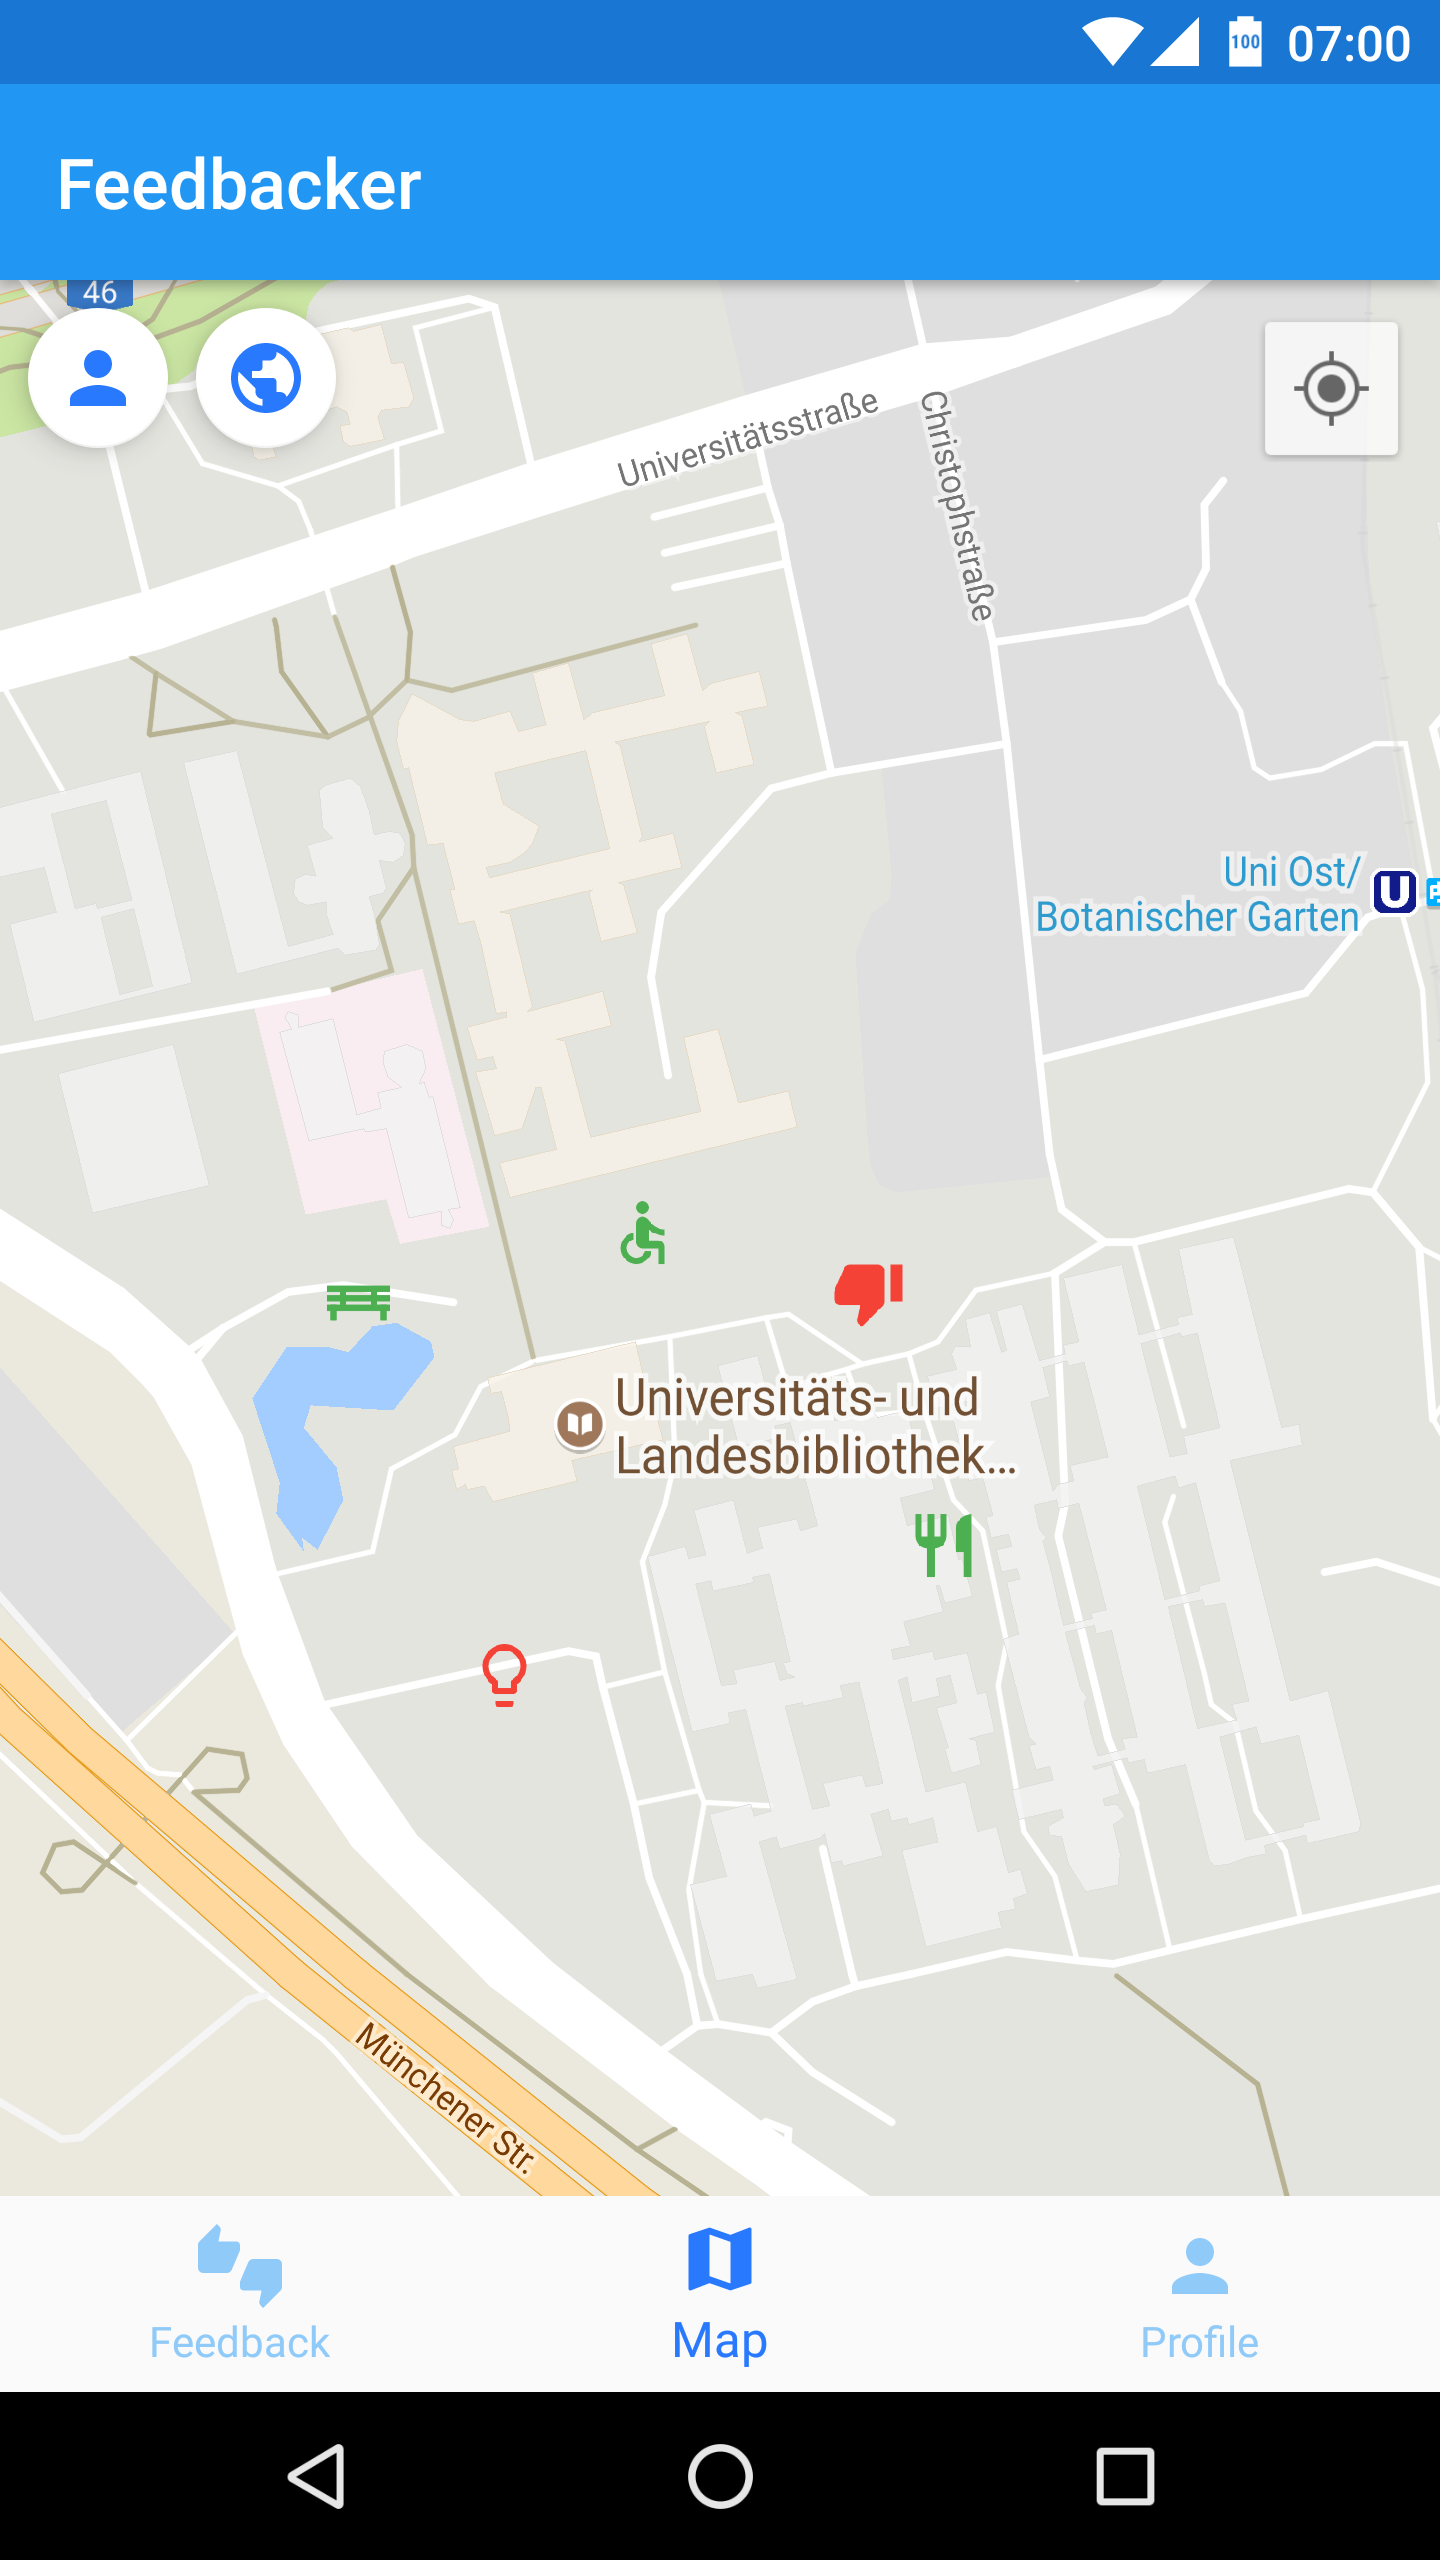
\includegraphics[width=\linewidth]{bilder/Screenshot_Map.png}
  \caption{Map View Android}\label{fig_map}
\endminipage\hfill
\minipage{0.32\textwidth}%
  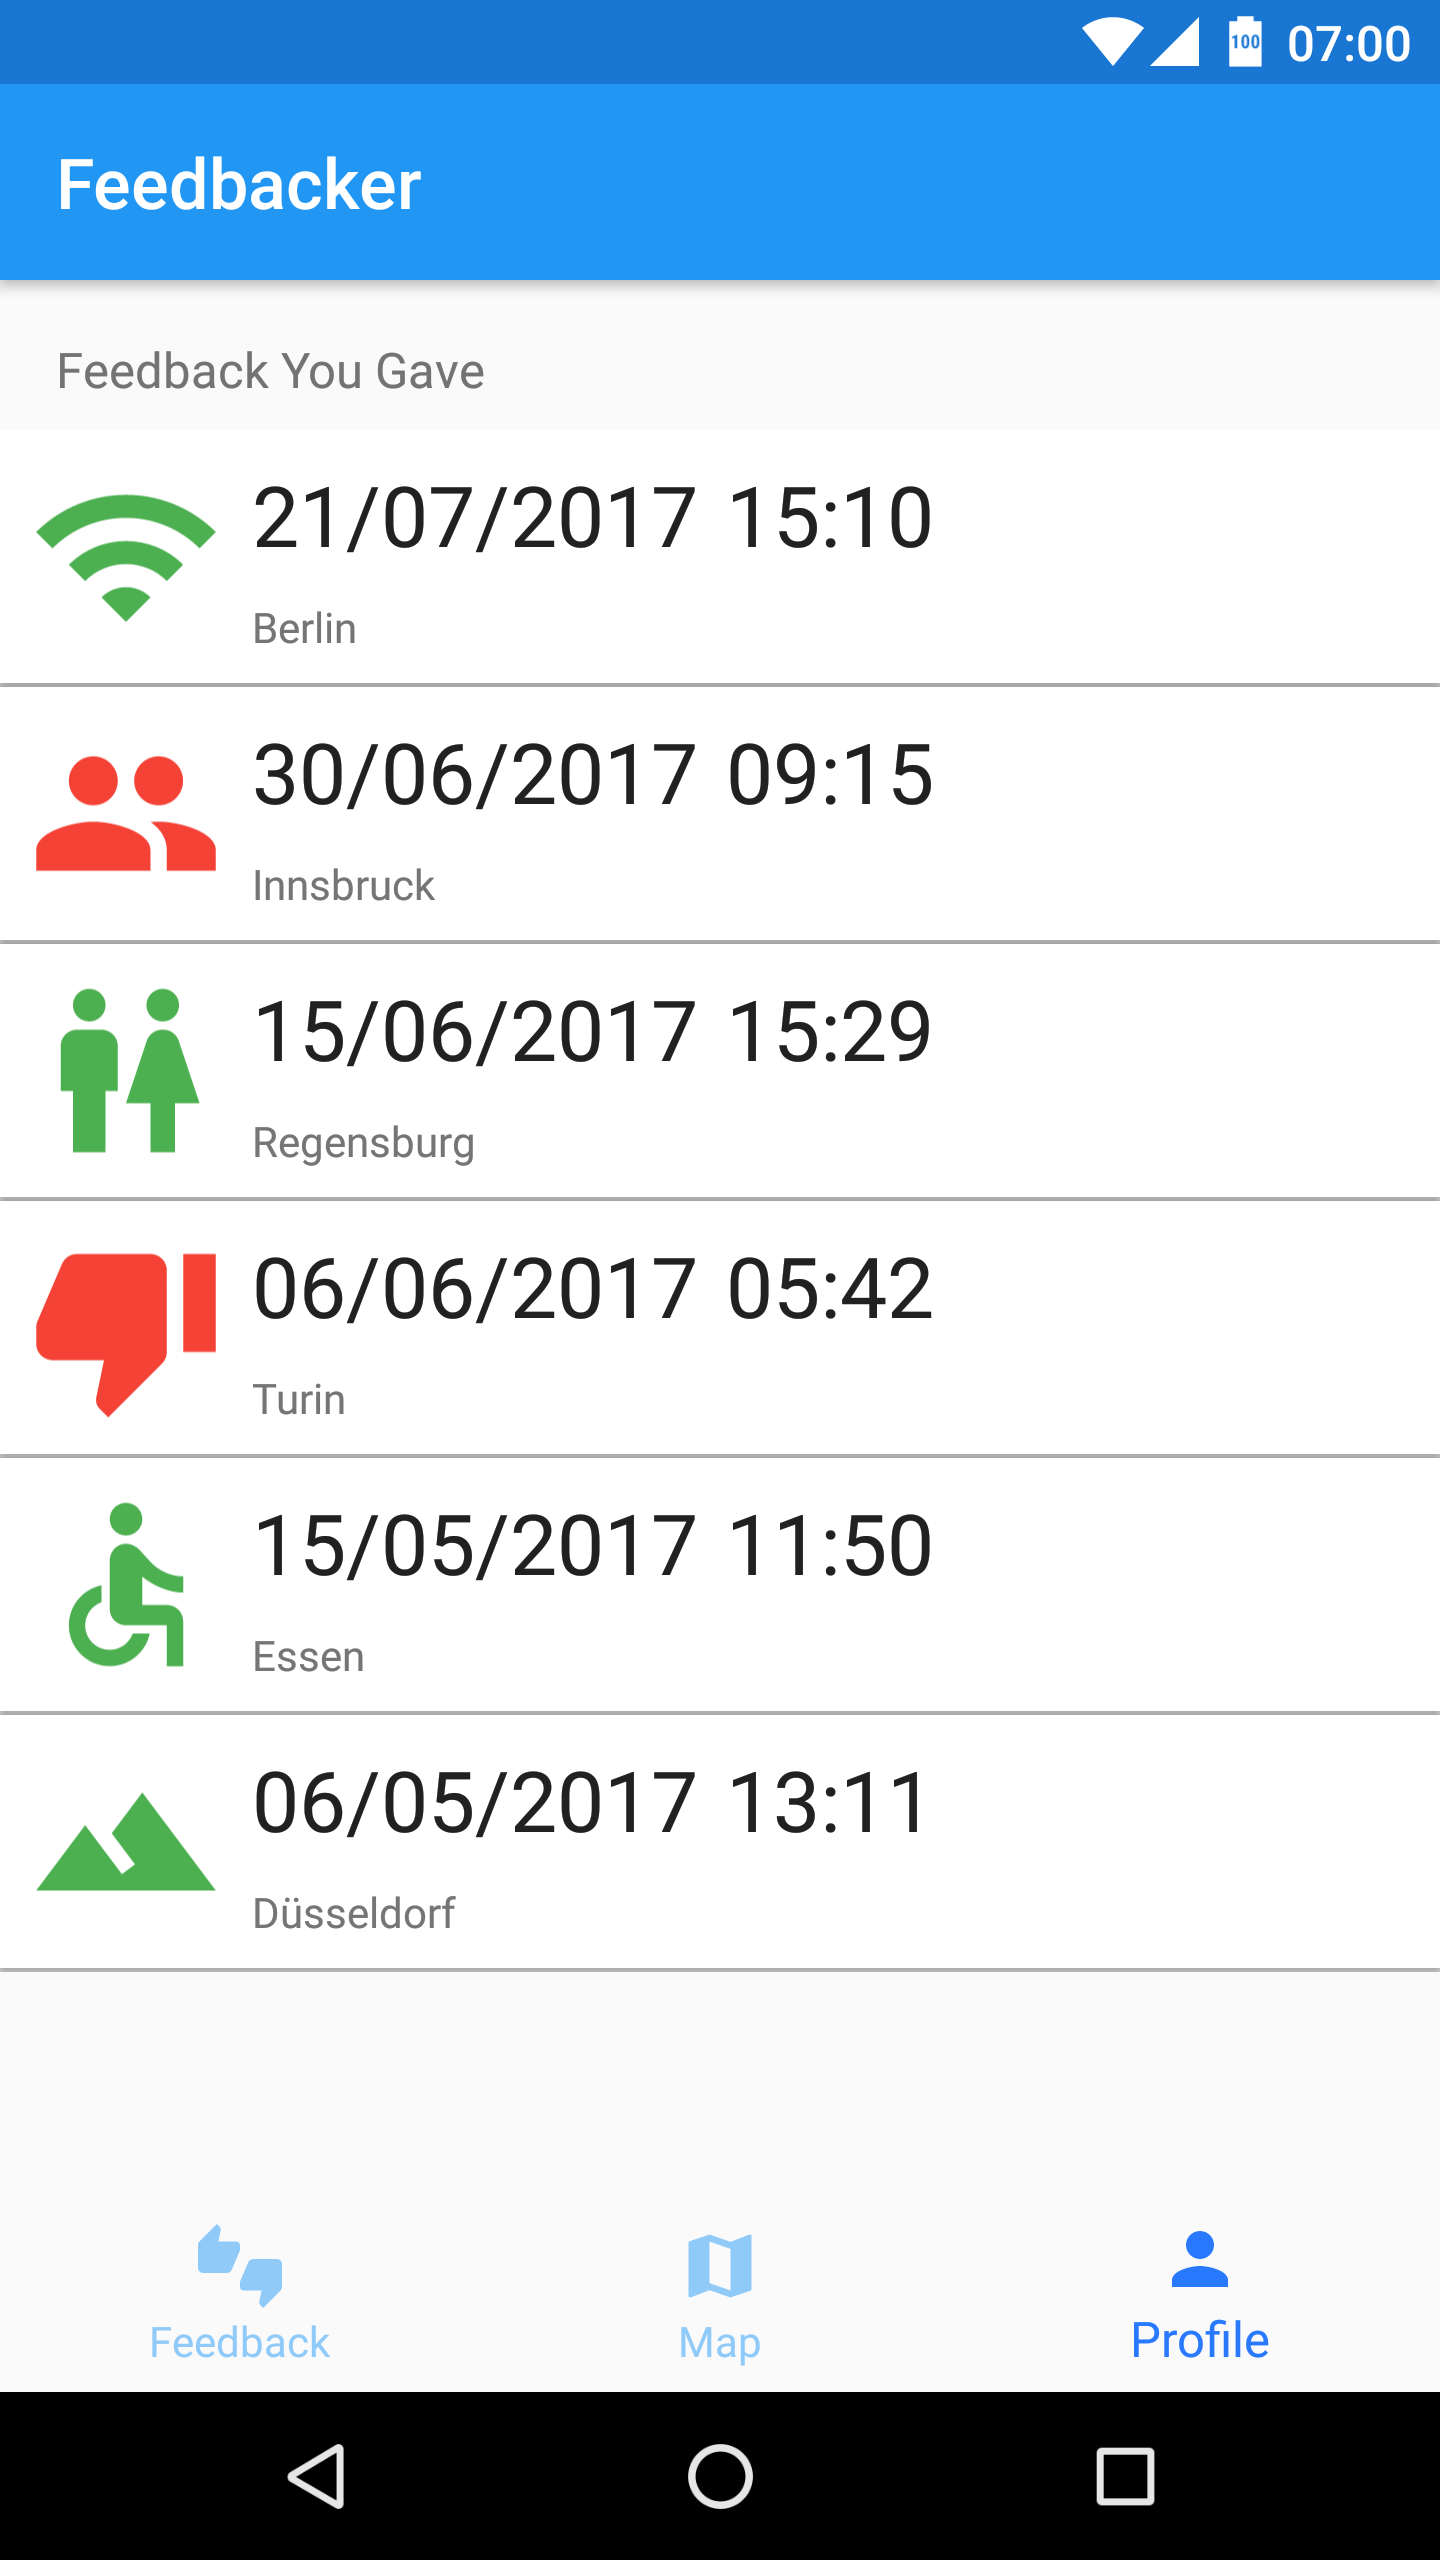
\includegraphics[width=\linewidth]{bilder/Screenshot_Profile.png}
  \caption{Profile View Android}\label{fig_profile}
\endminipage
\end{figure}

\subsubsection{Feedback View} \label{ssec:send}
This only displays two button to send positive and negative feedback, respectively. Clicking on either of these buttons will send a feedback of that type.


\subsubsection{Map View} \label{ssec:map}
This view displays a map with markers at the locations where feedback has been sent. Clicking on a Marker will open a popup with time and date of the feedback as well as the descriptive text if the feedback's sender provided one. Feedbacks provided by the user itself have a button to edit this feedback. \newline
In the top left corner there are buttons that allow the user to choose whether personal feedbacks and public feedbacks provided by other users should be displayed on the map.


\subsubsection{Profile View} \label{ssec:profile}
This view shows a list of the feedbacks provided by the user. Each feedback item has an icon based on the feedback's category as well as the time, date and city of that specific feedback.


\subsection{Feedback Edit View}
This view gives the user the ability to edit a feedback. This view can be reached via three ways. By sending a new feedback, via a marker on the map and from the list in the profile view. \newline

\begin{figure}[H]
  \begin{center}
    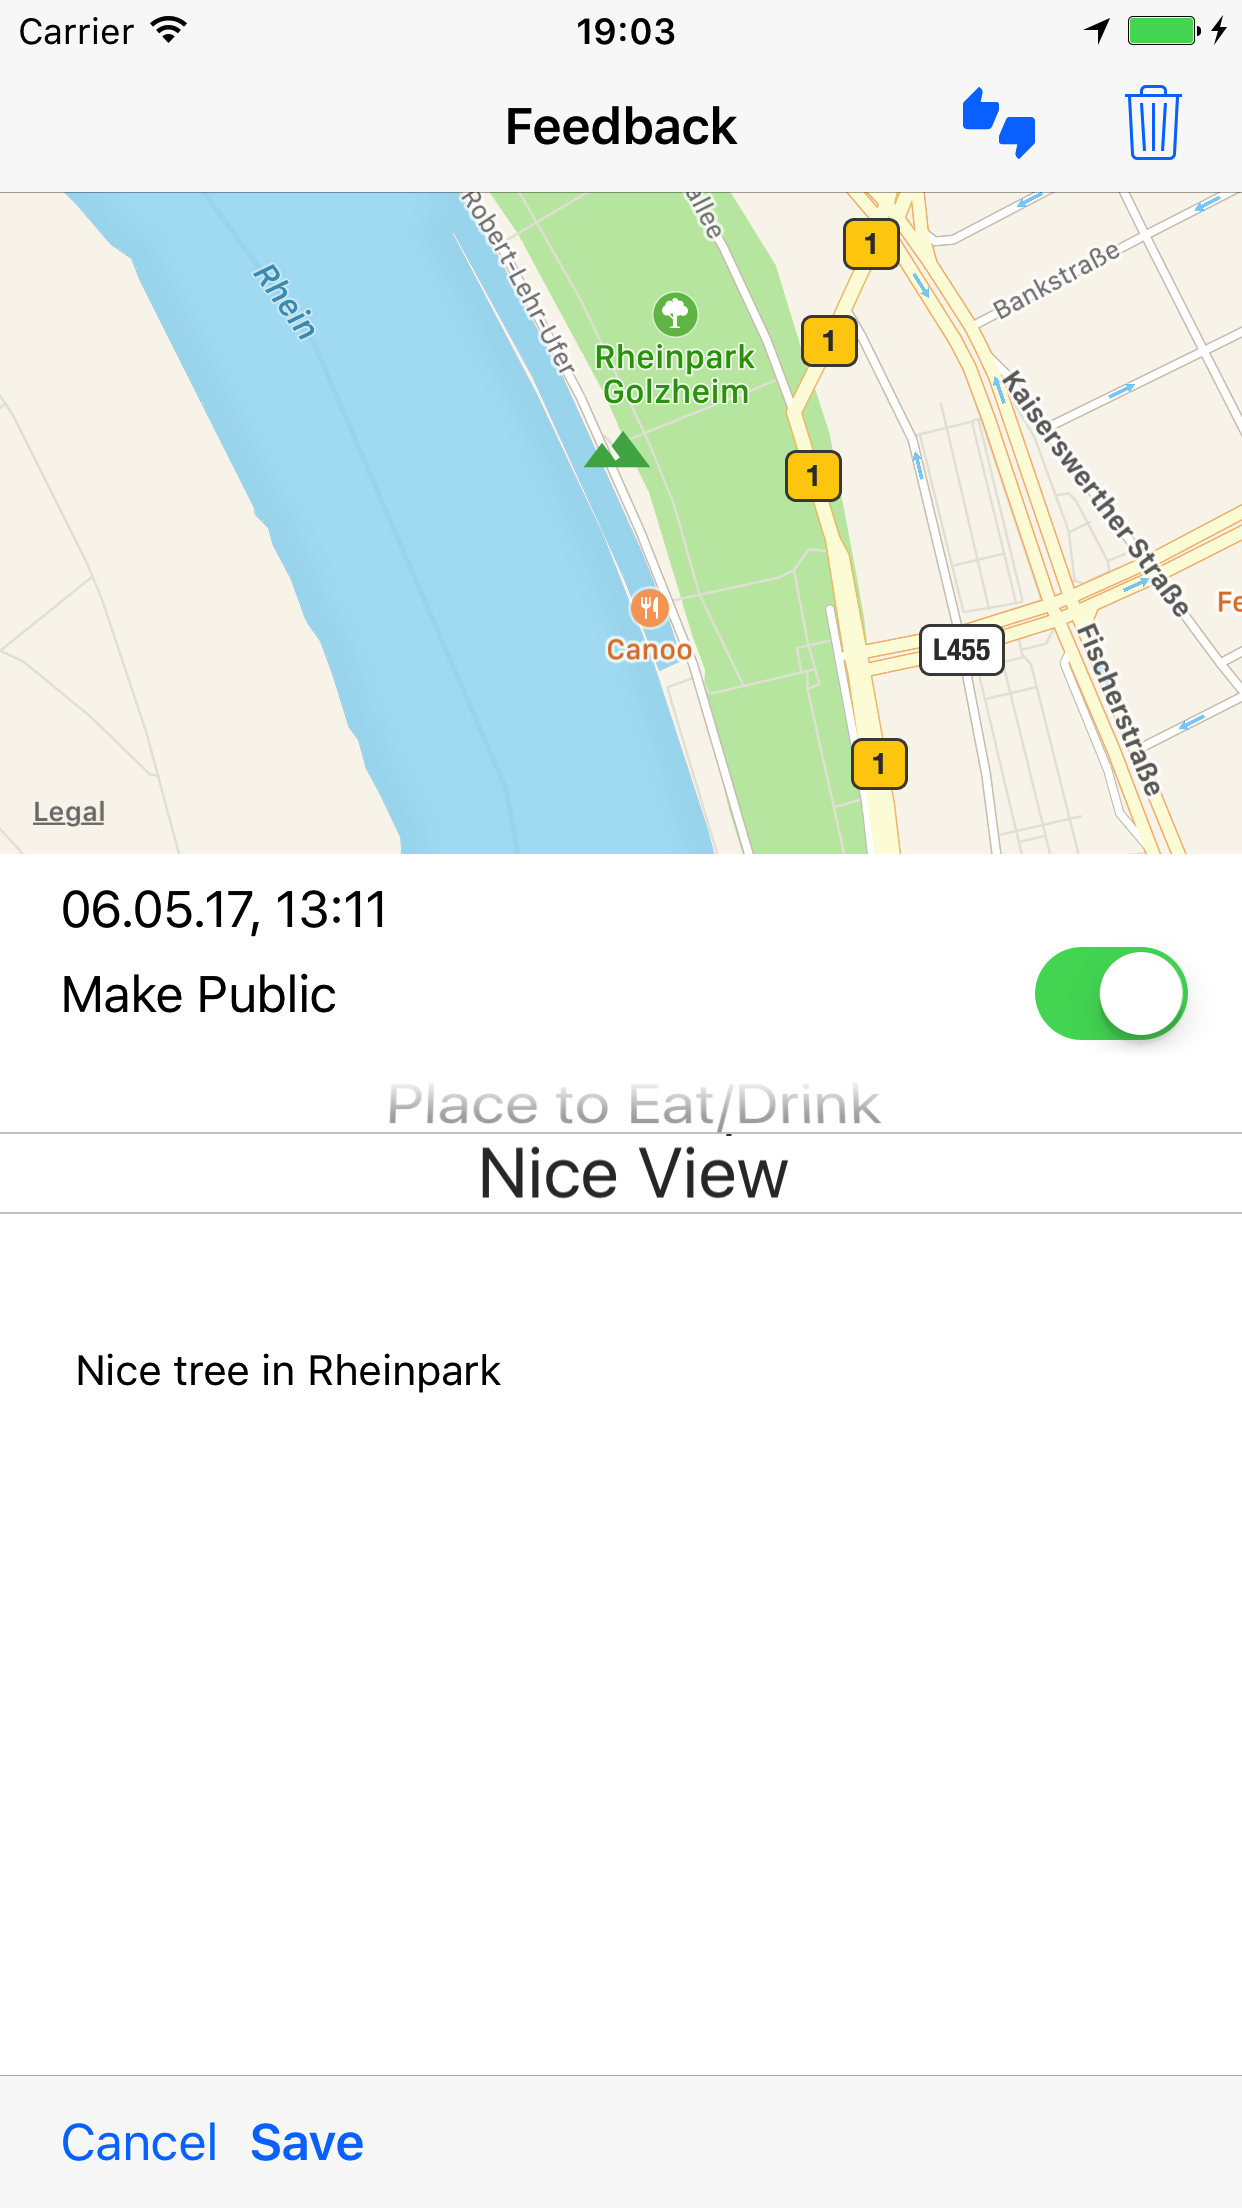
\includegraphics[width=0.32\textwidth]{bilder/Screenshot_Edit}
    \caption{Feedback Edit View iOS}\label{fig_edit}
  \end{center}
\end{figure}

\paragraph{View Components}
At the top of the layout there is a map marking the location of the feedback to give the user an orientation where his feedback is placed on the map. Directly below the date and time at which the feedback has been sent is shown. These features are common to all types of feedbacks, as they are send directly when the user hits one of the send feedback buttons. \newline
A switch can be used to mark the feedback as public, which will display that feedback for other users on the map. By default the switch is off. \newline
The category can be chosen from a menu. Depending on the kind of feedback (positive/negative), the menu will show the corresponding options listed in Table \ref{table:categories} on page \pageref{table:categories}. At the bottom of the layout there is a textbox for the user to provide a descriptive text for the feedback.

\paragraph{Toolbar Actions}
At the upper toolbar the user can switch the kind of the feedback as well as delete the feedback. Both of these actions will show a popup to confirm this action as they delete the currently selected category or the whole feedback, respectively. \newline
At the bottom there is a save and a cancel button. The save button will save all the edits the user has made to his feedback and the cancel button will discard all edits.

\section{Firebase}

\subsection{What is Firebase?}
Firebase is a platform of development tools for mobile and web apps.\\
It was originally founded by James Tamplin and Andrew Lee on September 1, 2011 \cite{crunchbase}. The first beta version was made available on April 21, 2012 \cite{beta}. Firebase was acquired by Google on October 21, 2014 \cite{crunchbase}.\\
Firebase's products can be separated into tools for development and tools for user growth and monetization. Feedbacker does not implement any features from the second category yet. The following table lists the features provided by Firebase that are used within the Feedbacker app.
\begin{table}[H]
\begin{center}
\begin{tabular}{l  l}
  Feature & used in Feedbacker \\
  \hline
    Realtime Database & Yes \\
    Crash Reporting & Yes \\
    Authentication & Yes \\
    Cloud Functions & No \\
    Cloud Storage & No \\
    Hosting & No \\
    Test Lab for Android & No \\
    Performance Monitoring & No \\
\end{tabular}
 \caption{Firebase Products}\label{tab_products}
 \label{table:products}
\end{center}
\end{table}

Most of Firebase's products offer support for Android, iOS, Web (in form of JavaScript), C++ and for Unity \cite{products}.



\subsection{Why Firebase for Feedbacker}
The primary reason for using firebase as the backend service was the ease of use for multiplatform development as well as the quick set-up which does not require to develop code for the server and the database. With Firebase it was easy to develop a first prototype which could then be refined, developed further and made more secure. \\
Also Firebase has all features which are necessary for Feedbacker, most importantly the database. Thinking ahead, many of possible features (see  section \ref{sec:future}) can be realized using Firebase.

\subsection{Authentication} \label{sec:auth}
Feedbacker makes use of Firebase's Anonymous Auth. This has the advantage that the user does not need to sign up with an email or similar form of authentication, skipping the signup/login step while still providing security and ensuring anonymity.
\begin{listing}
  \caption{User Authentication on Android}
  \label{mint:auth_android}
  \begin{minted}[frame=lines, framesep=10pt]{java}
FirebaseAuth auth = FirebaseAuth.getInstance();
if (auth.getCurrentUser() == null) {
  auth.signInAnonymously();
}
  \end{minted}

\end{listing}

This code checks whether or not the user is currently authenticated. If he is not, he will get signed in anonymously. Firebase will assign a random, unique UID for the user. Having a form of authentication is important to make the data in Firebase secure, as will be further explained in section \ref{ssec:sec_rules}

\subsection{Data Structure}\label{ssec:data_structure}
The firebase database stores the data in one JSON tree. The different sections within this JSON tree are explained in the following.

\paragraph{Categories}\label{par:db_cat}
All accepted categories are stored in the database to enable a security check (\ref{ssec:sec_rules}) when writing new feedback to the database.
\begin{listing}[H]
  \caption{Database Object Categories}
  \label{mint:db_categories}
  \begin{minted}[frame=lines, framesep=10pt]{json}
"categories" : {
  "NEG_DARK" : false,
  "NEG_DIRTY" : false,
  ...
  "POS_DISABILITY" : true,
  "POS_EAT_DRINK" : true,
  ...
}
  \end{minted}
\end{listing}
The allowed categories are stored as keys of a dictionary in the database. As only the keys are required for the security check, the values could be arbitrary. I chose to set them as a boolean value to make clear what kind of feedback the category is representing.


\paragraph{Feedback}
The most important objects in the database are those representing a single feedback (see the following example).
\begin{listing}[H]
  \caption{Database Object Feedback}
  \label{mint:db_feedback}
  \begin{minted}[frame=lines, framesep=10pt]{json}
"-KmSCGPr2UfcRHXpEPzo" : {
  "category" : "POS_EAT_DRINK",
  "city" : "Düsseldorf",
  "date" : 1497286119952,
  "details" : "Coffee at Campus Vita",
  "latitude" : 51.1921476,
  "longitude" : 6.793424,
  "positive" : true,
  "published" : false,
  "id" : "-KmSCGPr2UfcRHXpEPzo"
}
  \end{minted}
\end{listing}
The title of the object is a unique key, that Firebase generated before initially saving it to the database. "category" specifies the feedback and must be a valid key defined in the category section. The "date" attribute is the UNIX-Timecode of the feedback. "details" stores the optional descriptive text the user used to further specify his feedback. The attributes "latitude" and "longitude" are the coordinates of the feedback. The "positive" attribute shows whether a feedback is positive or negative with true for positive feedbacks and false for negative feedbacks. The "published" attribute determines whether or not the user published his feedback for other users.

\paragraph{User}
To allow only the creator of a feedback to edit it afterwards it is important to store the connection between each feedback and its creator in the database. The feedbacks are stored in a dedicated section in case more user data has to be sored separately in a future version of Feedbacker.
\begin{listing}[H]
\caption{Database Object User}
\label{mint:db_user}
\begin{minted}[frame=lines, framesep=10pt]{json}
"Vd2dbO95K7fT1PbzFt9ZnbDkLtz2" : {
  "feedback" : {
    "-Kmg08cxhJJ-bFJPWQGZ" : "POS_SIT",
    "-Kmg1KCc81FxAX__Zg_Q" : "NEG_GENERAL",
    "-Kmg1Qwx0e-pD0WPa-2f" : "NEG_DARK",
    "-Kmg1VFcJ_J6biXJDwhc" : "POS_VIEW"
  }
}
    \end{minted}
\end{listing}

The title of the section is the users unique UID, generated by Firebase during the authentication process (section \ref{sec:auth}). The feedback section holds keys that reference the unique IDs that are associated with each feedback this user has provided. The corresponding value details the category of the respective feedback. This allows updating the user interface (UI) in the map view and the profile view when the category changed.

\paragraph{Published}
All published feedbacks are stored in a section of the database as well.
\begin{listing}[H]
  \caption{Database Object Published}
  \label{mint:db_published}
  \begin{minted}[frame=lines, framesep=10pt]{json}
"published" : {
  "-KieONK1zQZueVvSIYIJ" : "POS_DISABILITY",
  "-KieWhBvNKZ7aZJr0YqJ" : "NEG_GRAFFITI",
  "-Klc-1KaHRvryB8LJiTn" : "POS_SIT",
  ...
}
  \end{minted}
\end{listing}

Similar to the user section, the individual feedbacks are stored with their unique ID and category, thus enabling to handle a change of category easily.



\subsection{Firebase Security Rules} \label{ssec:sec_rules}
An important part of every app handling sensitive data, like the user's location in this case, is the security of its database. In Firebase this is accomplished using security rules. They are necessary because, in contrast to a traditional database approach, all read and write operations are initiated by the user instead of the server. Therefore, read and write access as well as validating new data need to be handled by security rules.\\
The security rules work in a cascading way. This means that if a user has read or write access on one object of the database, he also has access on the children of that data object.

\paragraph{Category Level}
No rules have been specified for the category section. Firebase then automatically defaults the read and write access to false, which is a reasonable choice here. In the future it might be an option to allow admins write access in order to add new categories.


\paragraph{Feedback Level} \label{par:sec_rule_feedback}
As the app is built upon the feedbacks it is important to have them secured in the database. This is achieved by the following code.

\begin{listing}[H]
  \caption{Security Rules Feedback}
  \label{mint:sec_rule_feedback}
  \begin{minted}[frame=lines, framesep = 10pt, linenos, firstnumber=3, breaklines, breakbefore=.]{json}
"feedback":{
  "$feedbackID":{
    ".read" : "auth != null && (data.child('published').val() === true || root.child('users').child(auth.uid).child('feedback').child($feedbackID).exists())",
    ".write" : "auth != null && (!data.exists() || root.child('users').child(auth.uid).child('feedback').child($feedbackID).exists())",
    ".validate" : "newData.hasChildren(['latitude', 'longitude', 'positive', 'date', 'category', 'city', 'published', 'details', 'id'])",
    "latitude" : {".validate" : "newData.isNumber()"},
    "longitude" : {".validate" : "newData.isNumber()"},
    "positive" : {".validate" : "newData.isBoolean()"},
    "date" : {".validate" : "newData.isNumber()"},
    "category" : {".validate" : "newData.isString() && root.child('categories/' + newData.val()).exists()"},
    "city" : {".validate" : "newData.isString()"},
    "published" : {".validate" : "newData.isBoolean()"},
    "details" : {".validate" : "newData.isString()"},
    "id" : {".validate" : "newData.isString() && newData.val() === $feedbackID"},
    "$other" : {".validate" : false}
  }
},
  \end{minted}
\end{listing}

Line 5 handles who has read access on the Feedback. \mintinline{json}{"auth != null"} ensures that only users who are authorized (see section \ref{sec:auth}) have the possibility to read the data. \mintinline{json}{"data.child('published').val() === true"} grants read access if the feedback was published by another user. The rest of the expression checks if the feedback was send by the currently logged in user as \mintinline{json}{"auth.uid"} returns the uid of the user who makes the request.\\
The write access is handled similarly. It also checks if the user is authorized and if the request is coming from the author of feedback in case it is edited (Firebase does not distinguish between new writes and edits). For new data that is not yet written in the user's section \mintinline{json}{"!data.exists()"} allows this data to be saved. Line 7 is responsible for the sanity of new data. Specifically it checks whether a new data set has all the required fields. If it does not have all the fields, the write operation is cancelled and no data is written.\\
The other lines make sure only data of the correct type can be written in each field. For the category \mintinline{json}{"root.child('categories/' + newData.val()).exists()"} makes sure the category written is listed in the category section of the database.\\
To make sure the id saved really is the true id of the feedback \mintinline{json}{"newData.val() === $feedbackID"} is checked. As a last check \mintinline{json}|"$other" : {".validate" : false}| is making sure that all other fields are rejected and thus not writing to the database.


\paragraph{Published} \label{par:sec_rule_pub}
The security rules for the published section are less complicated.
\begin{listing}[H]
  \caption{Security Rules Published}
  \label{mint:sec_rule_published}
  \begin{minted}[frame=lines, framesep = 10pt, linenos, firstnumber=24, breaklines, breakbefore=.]{json}
"published":{
  "$publishedID":{
    ".read" : "auth != null",
    ".write" : "auth != null && root.child('users').child(auth.uid).child('feedback').child($publishedID).exists()",
    ".validate" : "newData.isString() && root.child('categories/' + newData.val()).exists()"
  }
},
  \end{minted}
\end{listing}

As the creators of the feedbacks in the published section are fine with other users seeing these feedbacks the only condition for read access is a successful authentication. For the write access it checks if the feedbackID is also in \textit{users/uid/feedback} to only allow authors of that feedback to make it public. The validation checks if the data is a string and is an entry in the category section.

\paragraph{Users}
Protecting the user data is also vital to ensure trust of the users.
\begin{listing}[H]
  \caption{Security Rules User}
  \label{mint:sec_rule_users}
  \begin{minted}[frame=lines, framesep = 10pt, linenos, firstnumber=24, breaklines, breakbefore=.]{json}
"users":{
  "$userID":{
  	".read" : "auth != null && $userID === auth.uid",
  	".write" : "auth != null  && $userID === auth.uid",
    "feedback" : {
      "$feedbackID" : {".validate" : "newData.isString() && root.child('categories/' + newData.val()).exists()"
      }
    },
    "$other" : {".validate" : false}
  }
}
  \end{minted}
\end{listing}

For read and write access it is checked whether the current user is authenticated in general. Furthermore \mintinline{json}|"$userID === auth.uid"| checks if the directory the request is made in belongs to the current users, thus making sure that a user can only read and write in his section.\\
Similar to the published rules (\ref{par:sec_rule_pub}) the validation of new data checks if the value is an entry from the cateogry section (\ref{par:db_cat}). Like rules for the feedback section data other than a feedback object are rejected and lead to an abortion of the write operation.

\subsection{Managing}
Firebase offers a web-based console to manage a Firebase project. It can be reached via \url{console.firebase.google.com}
On the main page it shows crash reports and usage numbers of the apps linked to that project. In the Authentication section the allowed forms of authentication can be set up. In case of Feedbacker this only allows anonymous auth.\\
In the database section the data is displayed. It also offers the possibility to export the data as JSON or importing existing data as JSON. Here there is also the section to edit the security rules (see section \ref{ssec:sec_rules}).\\
Other Firebase features (Table \ref{tab_products}, Page \pageref{tab_products}) can also be configured from the console.

\section{Multiplatform Development}
One of the goals of this thesis project was to develop an app that supports both iOS and Android. This section describes implementation details specific to the respective operating systems.
\subsection{Tools used \& supported Versions}
\paragraph{Android}
The Android App is written in Java using Android Studio as the development environment.\\
The minimum required Version of Android is API Level 16. This minimum Version Number determines which devices can run the App. As of July 6, 2017 this will mean that 98,6\%~\cite{versions_Android} of all Android Users can download, install and run the App.
\paragraph{iOS}
The iOS Version was developed in Xcode using Swift. The UI was developed with a storyboard which "is a visual representation of the user interface of an iOS application, showing screens of content and the connections between those screens" \cite{story}.\\
Feedbacker on iOS supports all devices running iOS 9 or newer. This corresponds to 97\% of all App Store users \cite{versions_iOS}.

\subsection{Implementation of Firebase}\label{ssec:implementation}

\subsubsection{Initialization}
For both platforms Firebase has to be imported as an additional library. Furthermore the \textit{google-services} file needs to reside in the app's directory. This file can be downloaded after registering the app in the firebase console.\\

\paragraph{Android}
Importing Firebase on Android is achieved by adding the relevant Firebase dependencies to the gradle build file. Also the Google Play Services plugin needs to be applied.
\begin{listing}[H]
  \caption{Gradle Dependencies}
  \label{mint:grdl_dep}
  \begin{minted}[frame=lines, framesep=10pt, breaklines=true, breakbefore=.]{groovy}
dependencies{
  compile 'com.google.firebase:firebase-core:10.2.1'
  compile 'com.google.firebase:firebase-database:10.2.1'
  compile 'com.google.firebase:firebase-auth:10.2.1'
  ...
}
apply plugin: 'com.google.gms.google-services'
  \end{minted}
\end{listing}

\paragraph{iOS}
iOS manages third party SDKs and dependencies with so called pods. They are configured inside a podfile and installed using \mintinline{bash}{pod install} in the command line. This will create a \textit{.xcworkspace} file which has to be used for further development.\\
After that was done successfully Firebase needs to be initialized inside the App Delegate with \mintinline{swift}{FirebaseApp.configure()}.

\subsubsection{Usage}\label{ssec:usage}
As explained in section \ref{ssec:data_structure}, Firebase saves data in a JSON tree. Each node in this tree can be addressed as a \textit{DatabaseReference}. The following examples show how read and write operations work in Firebase. As the APIs for Android and iOS are similar only the iOS version is shown here.

\paragraph{Read Data}
Firebase reads data by attaching an observer to a \textit{DatabaseReference}. The example below shows how this was used to mark the user's feedback on the Map (Figure \ref{fig_map}).\\

\begin{listing}[H]
  \caption{Read Data}
  \label{mint:read_data}
  \begin{minted}[frame=lines, framesep=10pt, breaklines=true, breakafter=)]{swift}
func createPersonalMarkers(){
  let uid : String = (Auth.auth().currentUser?.uid)!
  let personalFeedbackRef : DatabaseReference = FirebaseHelper.ref.child("users").child(uid).child("feedback")
  //Observe personal Feedback Ref for new Childs
  personalFeedbackRef.observe(.childAdded, with: { snapshot in
    let id : String = snapshot.key
    FirebaseHelper.ref.child("feedback").child(id).observeSingleEvent(of: .value, with: { (snapshot) in
      //Create Feedback from snapshot and create Annotation
    })
  })
  //Observe personal Feedback Ref for changes
  personalFeedbackRef.observe(.childChanged, with: { snapshot in
    let id : String = snapshot.key
    FirebaseHelper.ref.child("feedback").child(id).observeSingleEvent(of: .value, with: { (snapshot) in
      //Create Feedback from snapshot and create Annotation
    })
  })
  //Observe personal Feedback Ref for new deleted Childs
  personalFeedbackRef.observe(.childRemoved, with: {snapshot in
    let id : String = snapshot.key
    // Code for deleting the marker
  })
}
  \end{minted}
\end{listing}

The way the data is structured for Feedbacker (see section \ref{ssec:data_structure}) the user only saves a reference to a feedback in his section of database. This means that when an object was added or changed the corresponding feedback needs to be read as well. This is also achieved by observing a \textit{DatabaseReference} for the selected feedback. It is a one-time-only meaning it only reads the data once and then it is detaching itself from the reference.\\
When a user toggles to not show his personal feedback (or published feedbacks) on the map the observer on the reference is detached. This system of permanent observers and one time only observers means that the network traffic for the user is kept at a minimum.


\paragraph{Write/Delete Data}
For both apps a FirebaseHelper class was written to save, delete feedback and create new IDs for Feedback. The following explains how this was achieved.

\begin{listing}[H]
  \caption{Save Feedback}
  \label{mint:save_feedback}
  \begin{minted}[frame=lines, framesep=10pt, breaklines=true, breakafter=)]{swift}
static func saveFeedback(feedback : Feedback){
  let uid : String = (Auth.auth().currentUser?.uid)!
  //Save Feedback in User Section
  ref.child("users").child(uid).child("feedback").child(feedback.id).setValue(feedback.category)
  //If made public save it in Published
  if(feedback.published){
    ref.child("published").child(feedback.id).setValue(feedback.category)
  } else{
    ref.child("published").child(feedback.id).removeValue()
  }
  //Save the Feedback itself
  ref.child("feedback").child(feedback.id).setValue(feedback.getDataAsDict())
}
  \end{minted}
\end{listing}
It is important to note that the feedback is saved in the user directory, the feedback directory, and, if it is published, in the published directory.

\begin{listing}[H]
  \caption{Delete Feedback}
  \label{mint:delete_feedback}
  \begin{minted}[frame=lines, framesep=10pt, breaklines=true, breakafter=)]{swift}
static func deleteFeedback(feedback : Feedback){
  let uid : String = (Auth.auth().currentUser?.uid)!
  ref.child("feedback").child(feedback.id).removeValue()
  ref.child("published").child(feedback.id).removeValue()
  ref.child("users").child(uid).child("feedback").child(feedback.id).removeValue()
}
  \end{minted}
\end{listing}
Similarly, references to the feedback need to be removed from all sections in the database when it is deleted.

\begin{listing}[H]
  \caption{Generate Feedback Id}
  \label{mint:create_feedback_id}
  \begin{minted}[frame=lines, framesep=10pt, breaklines=true, breakafter=)]{swift}
static func getFeedbackId() -> String {
  return ref.child("feedback").childByAutoId().key
}
  \end{minted}
\end{listing}
The Firebase \mintinline{swift}{childByAutoId()} is used to create IDs for feedbacks. According to the Firebase documentation, this command "generates a new child location using a unique key" \cite{autoID}. This means that every new feedback really has a unique ID and cannot be overridden by another user's feedback.

\subsection{Location}
\subsubsection{Location Permission}
In order to get access to the user's location data, both platforms demand apps to ask for permission by the user to do so.

\paragraph{Android}
Up until Android 6.0 (API 23) Permissions were granted on installation. This led to many users not installing certain apps due to uncertainty why apps would need access to services like location.\\

\begin{listing}[H]
  \caption{Android Manifest Location Permission}
  \label{mint:manifest_and}
  \begin{minted}[frame=lines, framesep=10pt, breaklines=true, breakbefore=.]{xml}
  <uses-permission android:name="android.permission.ACCESS_COARSE_LOCATION"/>
  <uses-permission android:name="android.permission.ACCESS_FINE_LOCATION"/>
  \end{minted}
\end{listing}
If an app wants to use certain features it has to define them in the app's manifest. As Feedbacker is targeting API Level 25 it needs to request permissions also at runtime. If the user already granted the permission nothing happens. If the user has yet to allow location access for the app a dialog is shown, prompting the user to grant location access.\\

\begin{listing}[H]
  \caption{Location Permission Android}
  \label{mint:loc_perm_and}
  \begin{minted}[frame=lines, framesep=10pt, breaklines=true, breakbefore=.]{java}
public void onRequestPermissionsResult(int requestCode, String[] permissions, int[] grantResults) {
  super.onRequestPermissionsResult(requestCode, permissions, grantResults);
  switch (requestCode) {
    case PERMISSION_LOCATION_REQUEST_CODE: {
      if (grantResults.length > 0 &&
        grantResults[0] == PackageManager.PERMISSION_GRANTED) {
        //Check if App has Hardware Permissions [True because of App Manifest]
          //then start Listening for Location Update
      } else {
        //Permission for Location was Denied
        // --> Switch To Error Fragment
      }
    }
  }
}
  \end{minted}
\end{listing}


\paragraph{iOS}
On iOS the Location Manager is in charge of handling location permissions.
\begin{listing}[H]
  \caption{Location Permission iOS}
  \label{mint:loc_perm_ios}
  \begin{minted}[frame=lines, framesep=10pt, breaklines=true, breakbefore=.]{swift}
let locationManager = CLLocationManager()
locationManager.requestAlwaysAuthorization()
locationManager.requestWhenInUseAuthorization()
  \end{minted}
\end{listing}
The Location Manager is requesting access to the location of the user. If the user has not granted permission yet or has revoked location access a dialog will prompt the user to give the app access to the location.
Furthermore the usage of location and the reasons for it have to be declared in the \textit{Info.plist} file.

\begin{figure}[H]
\begin{center}
  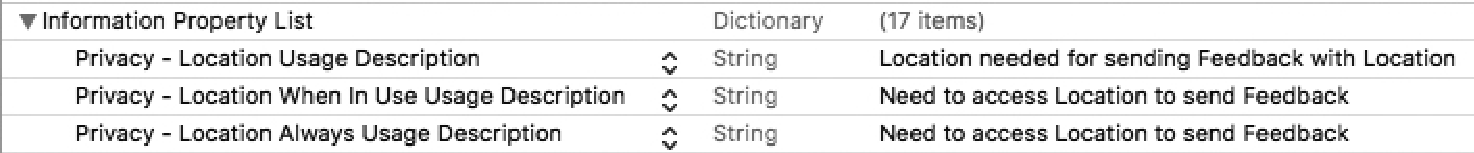
\includegraphics[width=400pt]{bilder/info_plist_location_bw.pdf}
  \caption{Location Permission flags in Info.plist}\label{infoplist_loc_perm}
\end{center}
\end{figure}


\subsubsection{Listening for Location Updates}
\paragraph{Android}
%%TODO: Link to GoogleApiClient and FusedLocationAPI Docs
Android's location updates are handled by a GoogleApiClient \cite{gAC} and the FusedLocationProviderAPI \cite{fla}.

\begin{listing}[H]
  \caption{Init Location Updates Android}
  \label{mint:loc_upd_and}
    \begin{minted}[frame=lines, framesep=10pt, breaklines=true, breakbefore=.]{java}
mLocationRequest = new LocationRequest();
//get new Location every 5-10 Seconds
mLocationRequest.setInterval(10000);
mLocationRequest.setFastestInterval(5000);
//Use highest Accuracy Possible
mLocationRequest.setPriority(LocationRequest.PRIORITY_HIGH_ACCURACY);
LocationSettingsRequest.Builder builder = new LocationSettingsRequest.Builder()
      .addLocationRequest(mLocationRequest).setAlwaysShow(true);
builder.build();
LocationServices.FusedLocationApi.requestLocationUpdates(mGoogleApiClient, mLocationRequest, this);
    \end{minted}
\end{listing}

First a location request is generated and configured (in this case with an update interval of 5-10 seconds, highest accuracy possible).

\begin{listing}[H]
  \caption{Location Changed Android}
  \label{mint:loc_changed_and}
    \begin{minted}[frame=lines, framesep=10pt, breaklines=true, breakbefore=.]{java}
@Override
public void onLocationChanged(Location location) {
  mCurrentLocation = location;
  mLastUpdateTime = Calendar.getInstance();
}
    \end{minted}
\end{listing}

This function is overridden from \mintinline{java}{com.google.android.gms.location.LocationListener} and is called every time the location changed.\\
If the location changed, the new location and the current time of the user's device will be saved.This information is accessed when a new feedback is created.

\paragraph{iOS}
Similar to Android first the location manager from Listing \ref{mint:loc_perm_ios} gets configured as desired.
\begin{listing}[H]
  \caption{Init Location Manager iOS}
  \label{mint:loc_mgr_ios}
    \begin{minted}[frame=lines, framesep=10pt, breaklines=true, breakbefore=.]{swift}
locationManager.delegate = self
locationManager.desiredAccuracy = kCLLocationAccuracyNearestTenMeters
locationManager.startUpdatingLocation()
    \end{minted}
\end{listing}

Also similar to Android a function is overridden to handle the callback when the location changed.
\begin{listing}[H]
  \caption{Location Changed iOS}
  \label{mint:loc_changed_ios}
    \begin{minted}[frame=lines, framesep=10pt, breaklines=true, breakbefore=.]{swift}
func locationManager(_ manager: CLLocationManager, didUpdateLocations locations: [CLLocation]) {
  let location = locations[0]
  coordinate = location.coordinate
  date = location.timestamp
}
    \end{minted}
\end{listing}
This function is implemented from \mintinline{swift}{CLLocationManagerDelegate}. Like in Listing \ref{mint:loc_changed_and} the new location and time are saved and accessed when creating a new feedback.

\subsection{Internationalization}
In order to give users the best experience possible it is best practice in App development to offer the App in as many Languages as possible. Both platforms Android and iOS achieve this by storing the strings to be displayed in the user interface in special language files.\\
The system then automatically chooses which string to pick and display to the user.\\
At the moment of releasing this thesis, Feedbacker supports English and German.

\paragraph{Android}
On Android the strings are saved in \textit{values/strings.xml} for the
standard translation (english) and in \textit{values-de/strings.xml} for german. Additional translations would be saved in a folder with the respective country code. This system also allows having different resource values like margins in layout for different regions.\\
\begin{listing}[H]
  \caption{Strings Android English}
  \label{mint:strings_and_eng}
    \begin{minted}[frame=lines, framesep=10pt, breaklines=true, breakbefore=.]{xml}
<string name="cat_neg_dark">Dark Place</string>
<string name="cat_neg_dirty">Dirty</string>
    \end{minted}
\end{listing}
The strings are identified by a key that is common to all languages implemented.
\begin{listing}[H]
  \caption{Strings Android German}
  \label{mint:strings_and_ger}
    \begin{minted}[frame=lines, framesep=10pt, breaklines=true, breakbefore=.]{xml}
<string name="cat_neg_dark">Dunkler Ort</string>
<string name="cat_neg_dirty">Dreckig</string>
    \end{minted}
\end{listing}
That is, the German strings all have the same key as the English counterparts with only the value changing according to the translation.\\


\paragraph{iOS}
iOS also utilizes special files to support different languages. The languages wanted have to be declared in the info section of the project settings.\\
This will then create \textit{*.string} files for the storyboard selected.\\
\begin{listing}[H]
  \caption{Strings iOS English}
  \label{mint:strings_ios_eng}
    \begin{minted}[frame=lines, framesep=10pt, breaklines=true, breakbefore=.]{java}
/* Class = "UITabBarItem"; title = "Map"; ObjectID = "cPa-gy-q4n"; */
"cPa-gy-q4n.title" = "Map";
/* Class = "UITabBarItem"; title = "Profile"; ObjectID = "kUv-uF-GHa"; */
"kUv-uF-GHa.title" = "Profile";
    \end{minted}
\end{listing}

Similar to Android all UI-Strings have a common key and the value according to the language.
\begin{listing}[H]
  \caption{Strings iOS German}
  \label{mint:strings_ios_ger}
    \begin{minted}[frame=lines, framesep=10pt, breaklines=true, breakbefore=.]{java}
/* Class = "UITabBarItem"; title = "Map"; ObjectID = "cPa-gy-q4n"; */
"cPa-gy-q4n.title" = "Karte";
/* Class = "UITabBarItem"; title = "Profile"; ObjectID = "kUv-uF-GHa"; */
"kUv-uF-GHa.title" = "Profil";
    \end{minted}
\end{listing}

The app will automatically display the UI with the language selected by the user in the system settings.\\
Localized strings required outside of the UI are saved in \textit{localized.string} similar to the storyboard and UI relevant files they get sub level files for each language. These Strings can be accessed project-wide with \mintinline{swift}{NSLocalizedString("cat_neg_dark", comment: NEG_DARK)}.

\section{Future of the App} \label{sec:future}

At the time of finishing this thesis, the app is functioning in the way described previously. However, there is still room for improvement both in the implementation and in the features of the app. In the following I list some possible improvements.

\subsection{Implementation enhancements}
\paragraph{Cloud Functions}
With the current version of the app, writing to and deleting from the database have to be done inside the app for all three database sections (see section \ref{ssec:usage}). This can lead to problems if an operation fails in one of the sections. A more elegant solution would be to perform only one operation in the app and handle the event accordingly inside Firebase's Cloud Functions (Table \ref{table:products}, Page \pageref{table:products}).
\paragraph{Error Handling}
At the moment not all errors are caught and handled accordingly. For example, when a user turns off the location services on his device, the Android version of the app will currently show an error screen. Ideally, a future version of the app would handle all errors in a similar way to ensure users the best possible experience.


\subsection{Feature Enhancements}
\paragraph{Pictures}
In order to make the feedbacks more detailed users could be given the possibility to upload a picture with their feedback. Especially for categories such as nice view or dirty places pictures could portray that feedback better than a text.\\
Firebase Storage would be an option to implement this.
\paragraph{Filtering in Maps}
At the moment it is possible to display the user's own feedbacks or public ones (or both). Future versions could offer more filtering options, like positive/negative or even category-specific (for example to only show places with a positive feedback with the "place to eat/drink" category when searching for a place to have dinner in an unknown city).


\subsection{New Features}
\paragraph{Social}
The anonymity of users is a left-over that is due to the original idea of developing an app that can be used to identify dangerous places.\\
A possibility might be to give the app a more social character. Social networks like Facebook, Instagram and Twitter belong to the most popular apps in the world. Concerning Feedbacker itself possible features could be commenting on feedback or following users to get notified when they send new feedback.\\
This could give businesses like shops and restaurants a possibility to contact people sending positive or negative feedback about their place directly in order to improve its perception.
\paragraph{Web Platform}
To visualize feedbacks outside of the app a website could be offered to allow people to display the feedbacks on a bigger screen.\\
This web platform could also be used by administrators to add categories.

\section{Conclusion}
This work documents the process of developing a multiplatform, location-based app called Feedbacker.\\
\paragraph{Development Process}
The development process showed that Firebase is a great tool not only for developing an app with both Android and iOS support in general, but also for achieving this quickly and efficiently.\\
Especially when working with database-focused apps like Feedbacker Firebase can play out its strengths. The simplicity of
While there are still many things that could be improved in the future, especially regarding the user interface in  the iOS version, this work showed that it is possible to develop functioning prototypes for two platforms in a relatively short amount of time.

\paragraph{Future}
The future of the app depends heavily on its success after being released in the Apple App Store and Google Play Store respectively.\\
The success should not only be measured by the number of installations but especially by usage numbers. As Feedbacker is a crowdsourcing app it relies on active users that send feedback regularly. It is also important that the group of active users is as big as possible. The value of the app might increase further if it is used by many people in the same region, thus resulting in a large density of feedbacks in that region. This effect might be achieved by investing in advertising the app in selected cities and communities.\\


%%%%%%%%%%%%%%%%%%%%%%%%%%%%%%%%%%%%%%%%%%%%%%%%%%%%%%%%%%%%%%%%%%%%%%%%
%%%% ENDE TEXTTEIL %%%%%%%%%%%%%%%%%%%%%%%%%%%%%%%%%%%%%%%%%%%%%%%%%%%%%
%%%%%%%%%%%%%%%%%%%%%%%%%%%%%%%%%%%%%%%%%%%%%%%%%%%%%%%%%%%%%%%%%%%%%%%%

\clearpage

% Entfernen Sie das Kommentar aus der nachfolgenden Zeile, falls Sie einen Anhang in der Arbeit verwenden wollen. Beachten Sie, dass Sie sich im Verlauf der Arbeit mit \ref{...} (z.B. \ref{anhang:zusatz1}) auf den Anhang beziehen.
%\input{anhang}

\bibliography{references}
\bibliographystyle{alphadin}
%\vspace*{\fill}

\clearpage

\listoffigures

\listoftables

\listoflistings
\addcontentsline{toc}{section}{List of Listings}

\pagebreak
\thispagestyle{empty}

\begin{center}
  \vspace{-3cm}
  \fbox{\parbox[c][12cm][c]{12cm}{\centering Please add here\\[1cm] the CD holding sheet}}
\end{center}

\vfill

\textbf{This CD contains:}
\begin{itemize}
 \item A \emph{pdf} Version of this bachelor thesis
 \item All \LaTeX\ and graphic files that have been used, as well as the corresponding scripts
 \item The Android Studio Project of Feedbacker
 \item The Xcode Project of Feedbacker
 \item An APK of Feedbacker to install on Android Devices
\end{itemize}


%\pagebreak

%\printindex
\end{document}
